
Being a common tool in software development, CMake has integrations with a wide variety of IDEs and source code editors. Using such integrations while using an IDE or editor is perhaps more convenient for the user. In this section, we will cover how CMake integrates with some of the popular IDEs and editors.

If you are expecting a guide about how to use an IDE or editor, this section is not going to be about that. The main focus of this section is to investigate and learn about CMake integrations with such tools. This section assumes that you have existing experience with the IDE/editor you are going to interact with.

Let's start with Visual Studio.

\subsubsubsection{2.4.1\hspace{0.2cm}Visual Studio}

Visual Studio was one of the latecomers to the party when supporting CMake. Unlike other popular IDEs, Visual Studio had no native support for CMake until the year 2017. In that year, Microsoft decided to make a move and introduced built-in support for handling CMake projects, which is shipped Visual Studio 2017. Since then, it has been a solid feature of Visual Studio IDE.

To get started, obtain a copy of Visual Studio 2017 or later. For the older versions of Visual Studio, the feature is completely absent. In our examples, we'll be using Visual Studio 2022 Community Edition.

\hspace*{\fill} \\ %插入空行
\noindent
\textbf{Starting a CMake project from scratch}

The Visual Studio project creation feature is based on project templates. With VS2017 and upward, project templates contain a CMake project template as well. We are going to learn how to use this template to create new CMake projects.

To create a new CMake project with Visual Studio, click the Create a new project button on the welcome page. Alternatively, you can access it by clicking on File | New | Project on the main IDE window, or using the Ctrl + Shift + N (New Project) keyboard shortcut. The VS22 welcome screen looks like this:

\begin{center}
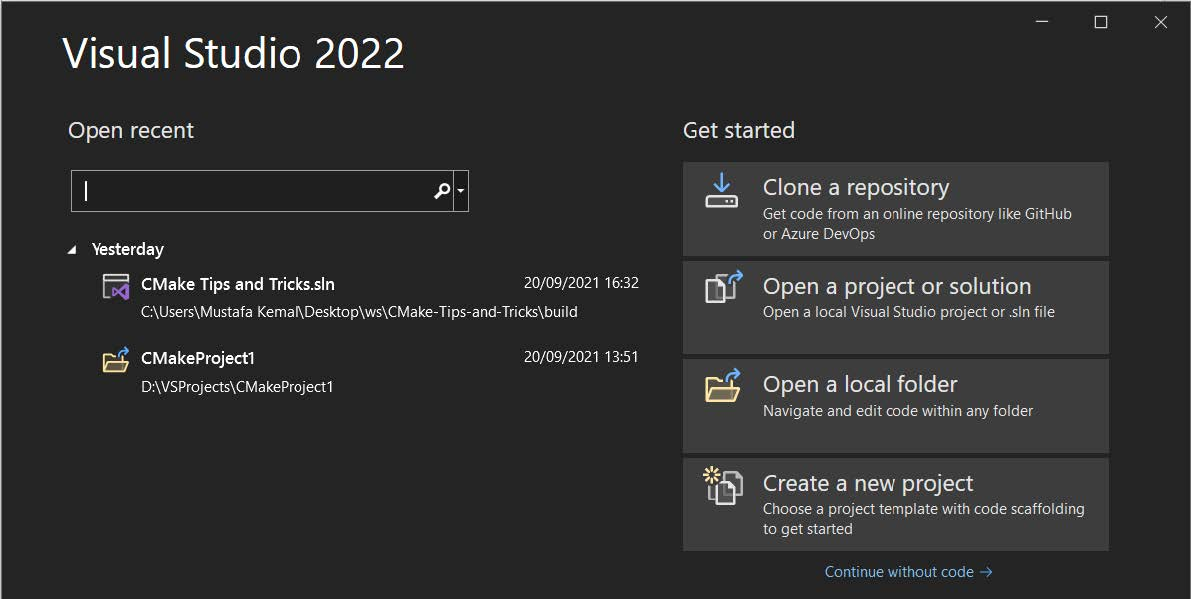
\includegraphics[width=0.8\textwidth]{content/1/chapter2/images/35.jpg}\\
Figure 2.35 – Visual Studio 2022 welcome screen
\end{center}

On the Create a new project screen, double-click on CMake Project in the project template list. You can filter project templates by using the search bar located at the top of the list:

\begin{center}
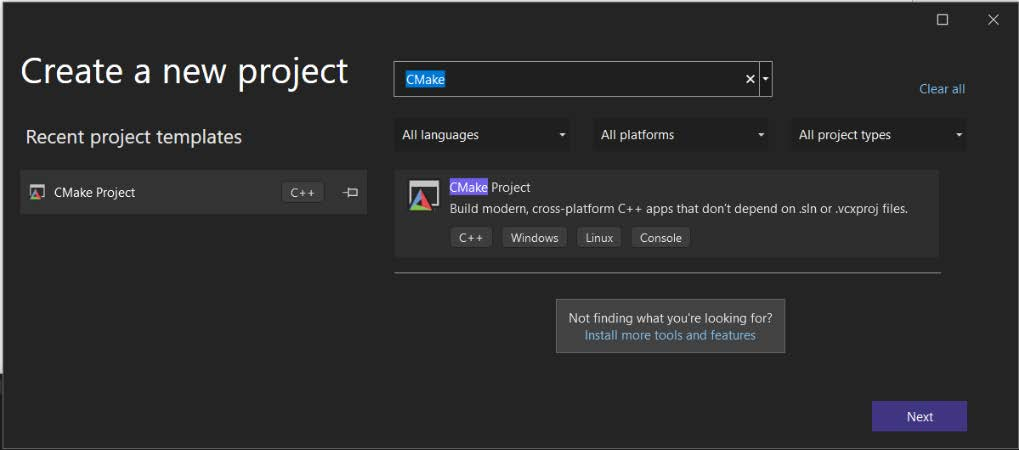
\includegraphics[width=0.8\textwidth]{content/1/chapter2/images/36.jpg}\\
Figure 2.36 – Visual Studio 2022 Create a new project screen
\end{center}

After clicking Next, the project configuration screen will appear. On this page, you can give your new CMake project a name and choose where to put your new project. In our example, we'll go with the default project name, CMakeProject1.

\begin{center}
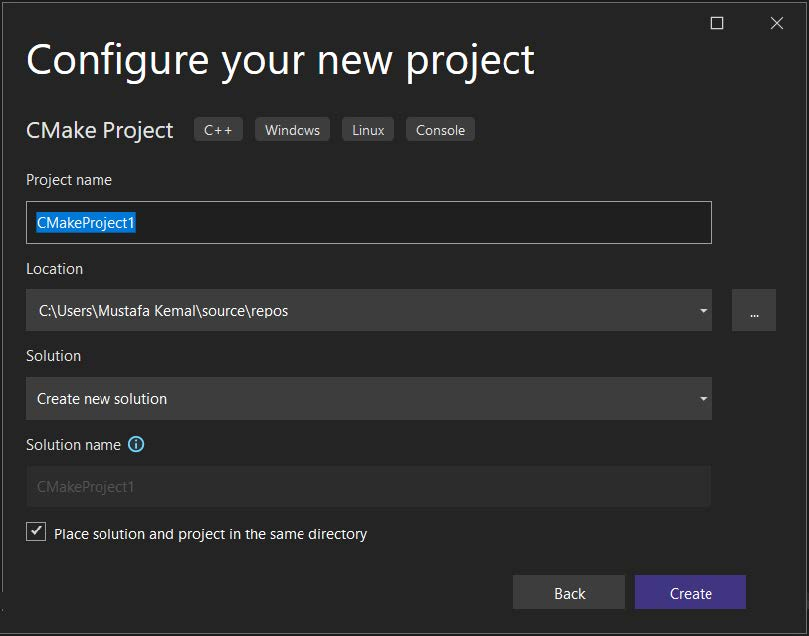
\includegraphics[width=0.8\textwidth]{content/1/chapter2/images/37.jpg}\\
Figure 2.37 – Visual Studio 2022 new project configuration screen
\end{center}

After filling in the details, click Create to create your new CMake project. The generated project will contain a top-level CMakeLists.txt file, a C++ source file, and a C++ header file, named after the chosen project name. The newly created project's layout can be seen in the following figure:

\begin{center}
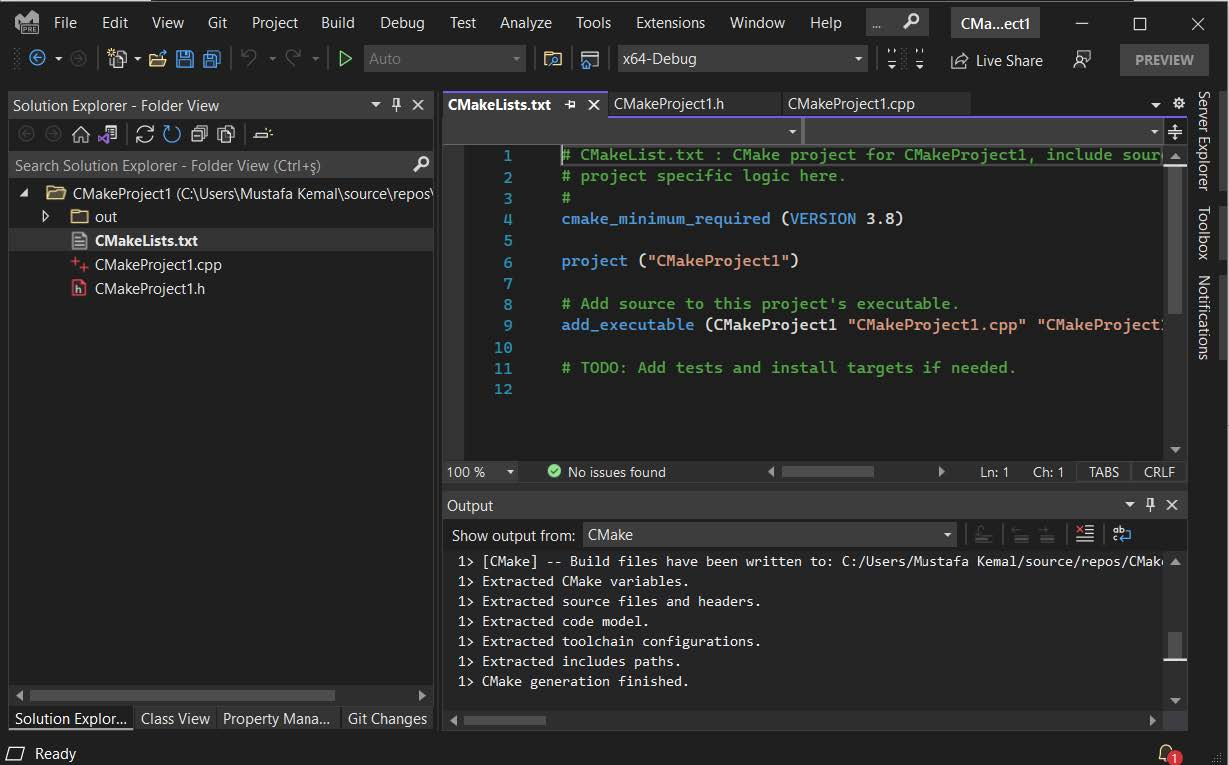
\includegraphics[width=0.8\textwidth]{content/1/chapter2/images/38.jpg}\\
Figure 2.38 – First glance after creating a new CMake project with Visual Studio
\end{center}

\hspace*{\fill} \\ %插入空行
\noindent
\textbf{Opening an existing CMake project}

To open an existing CMake project, go to File | Open | CMake... and select the top-level CMakeLists.txt file of the project to be opened. The following figure shows what the Open menu looks like:

\begin{center}
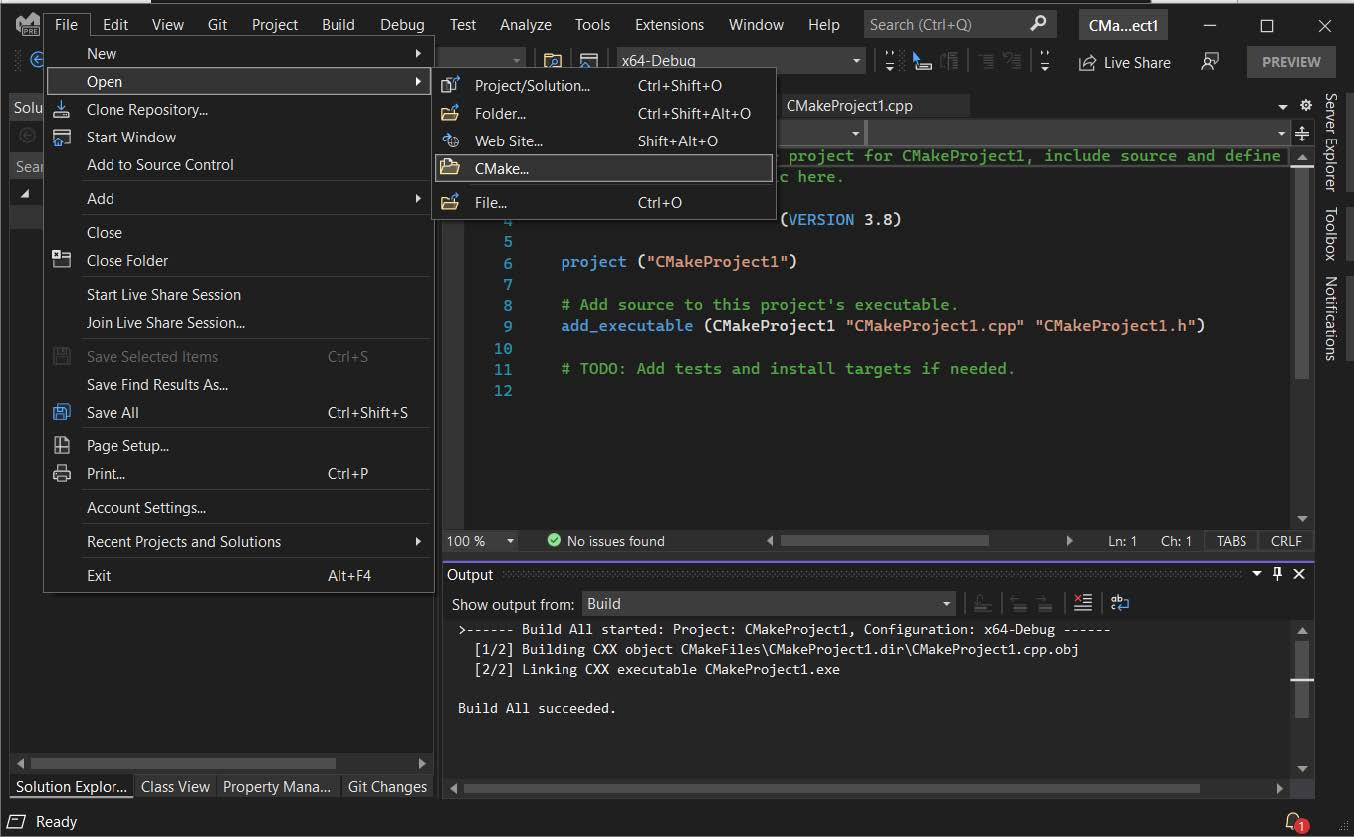
\includegraphics[width=0.8\textwidth]{content/1/chapter2/images/39.jpg}\\
Figure 2.39 – CMake project open menu
\end{center}

Next, let's see how a CMake project can be configured and built.

\hspace*{\fill} \\ %插入空行
\noindent
\textbf{Configuring and building a CMake project}

To build a CMake project in Visual Studio, go to Project | Configure first. This will invoke the CMake configure step and generate the required build system files. After configuration, click Build | Build All to build the project. You can also trigger Build All by using the F7 keyboard shortcut.

Note that Visual Studio will automatically invoke configure whenever you save a CMakeLists.txt file, which is a part of the project.

\hspace*{\fill} \\ %插入空行
\noindent
\textbf{Executing common actions on a CMake target}

Visual Studio uses a startup target concept for target-requiring actions such as build, debug, and launch. To set a CMake target as a startup target, use the Select Startup Target drop-down box located on the toolbar. Visual Studio will automatically populate this drop-down box with Cmake targets on configuration.

\begin{center}
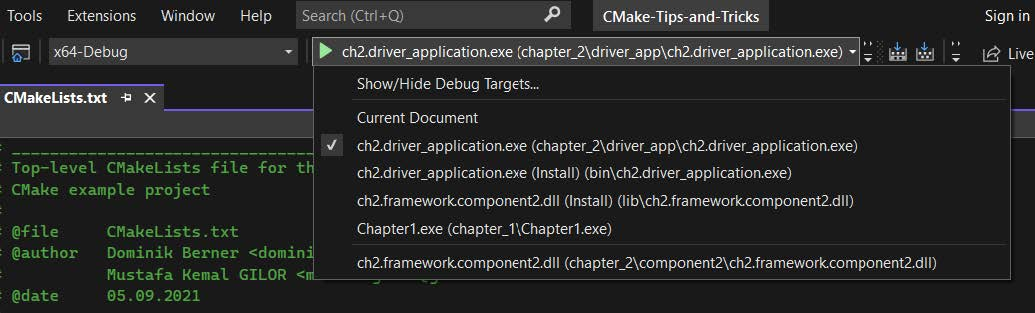
\includegraphics[width=0.8\textwidth]{content/1/chapter2/images/40.jpg}\\
Figure 2.40 – Startup target selection drop-down menu
\end{center}

After setting a startup target, you can invoke actions such as Debug, Build, or Launch, just as you always do in Visual Studio:

\begin{itemize}
\item 
To debug, first, click on Debug | Startup Target, and then click Debug | Start Debugging or use the F5 keyboard shortcut.

\item 
To start without debugging, click on Start without debug or use the Ctrl + F5 keyboard shortcut.

\item 
To build, click on Build, or click Build | Build <target>, or use the Ctrl + B keyboard shortcut.

\item
Button locations are shown in the following figure:

\begin{center}
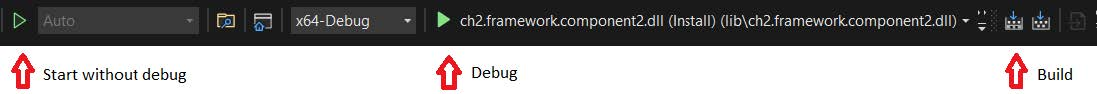
\includegraphics[width=0.8\textwidth]{content/1/chapter2/images/41.jpg}\\
Figure 2.41 – Toolbar button locations
\end{center}
\end{itemize}

In this section, we've covered the basics of the Visual Studio CMake integration. In the next section, we'll continue to learn with another Microsoft product, Visual Studio Code.

\subsubsubsection{2.4.2\hspace{0.2cm}Visual Studio Code}

Visual Studio Code (VSCode) is an open source code editor developed by Microsoft. It is not an IDE but can become powerful and have IDE-like features via extensions. The extension market has a wide variety of additional content, from themes to language servers. You can find an extension for pretty much anything, which makes VSCode both powerful and liked by a wide audience. With no surprise, VSCode has an official CMake extension too. This extension was originally developed by Colby Pike (also known as vector-of-bool) but it is now officially maintained by Microsoft. 

In this section, we are going to learn how to install the extension and perform basic CMake tasks using it.

Before going any further, VSCode must be already installed in your environment. If not, visit \url{https://code.visualstudio.com/learn/get-started/basics} for details on downloading and installing it.

Also, we will frequently access the Command Palette. It is strongly recommended to use it often to gain familiarity. For those asking What the heck is the Command Palette?, here is a screenshot:

\begin{center}
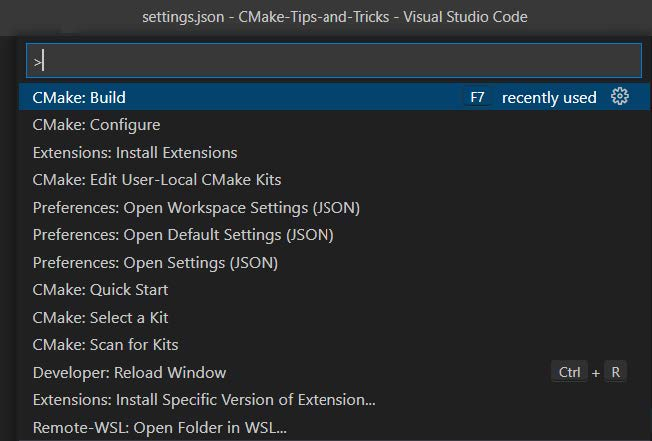
\includegraphics[width=0.8\textwidth]{content/1/chapter2/images/42.jpg}\\
Figure 2.42 – VSCode Command Palette
\end{center}

Yeah, it is that thing. To be honest, I did not know it had a name until now. Shortcuts for accessing the Command Palette are F1 and Ctrl + Shift + P. The Command Palette is the bread and butter of VSCode; it speeds up the VSCode workflow.

\hspace*{\fill} \\ %插入空行
\noindent
\textbf{Installing the extension}

Installing the extension is pretty straightforward and simple. To install it by using a CLI, invoke the following command (replace code with code-insiders if you're using the Insiders edition):

\begin{tcblisting}{commandshell={}}
code --install-extension ms-vscode.cmake-tools
\end{tcblisting}

Alternatively, you can do the same in the VSCode GUI as well. Open VSCode and navigate to the Extensions page by clicking Extensions on the left-side navigation pane. Alternatively, you can use the Ctrl + Shift + X shortcut. Type CMake Tools into the extension search box and select CMake Tools from Microsoft. Be careful not to confuse it with the CMake extension. Press the Install button to install it.

\begin{center}
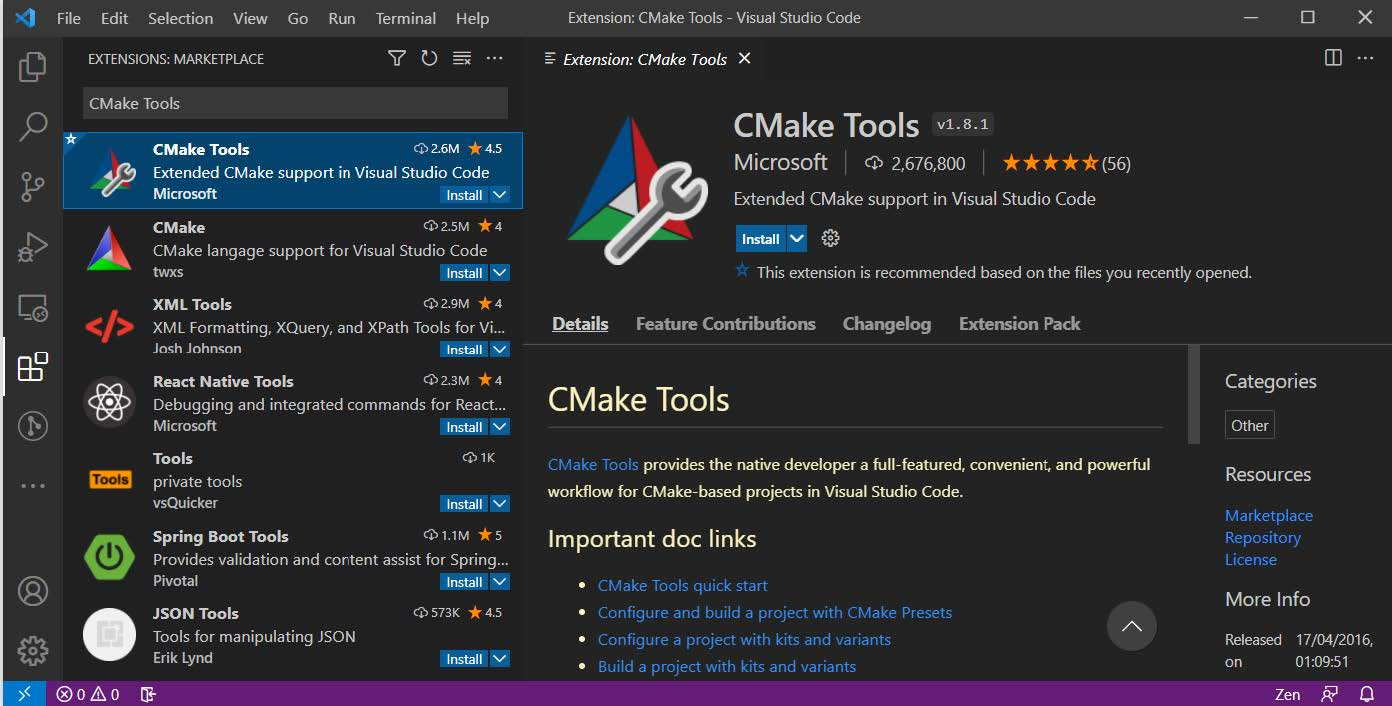
\includegraphics[width=0.8\textwidth]{content/1/chapter2/images/43.jpg}\\
Figure 2.43 – VSCode extensions marketplace
\end{center}

After installation completes, the extension is ready to use.

\hspace*{\fill} \\ %插入空行
\noindent
\textbf{Quick Start project}

The VSCode CMake Tools extension offers a Quick Start option that bootstraps a CMake project with example C++ code. To use it, first open the destination folder by using the File | Open Folder... menu, and then press F1 and type cmake quick start. Select CMake: Quick Start and press Enter on the keyboard.

\begin{center}
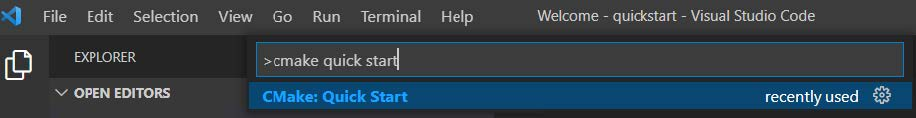
\includegraphics[width=0.8\textwidth]{content/1/chapter2/images/44.jpg}\\
Figure 2.44 – Command Palette – Locating CMake: Quick Start
\end{center}

Firstly, the extension will ask which kit to use. Select the one that is appropriate for your new project. Kits will be further discussed in the Dealing with kits section.

After selecting a kit, you will be asked to input a project name. This will be the name of your top-level CMake project. Enter a name of your choice.

Lastly, a choice for example application code will be shown. In this choice, you will be asked to create an executable application project or a library project. Select one, and voil•! You've got yourself a working CMake project. Upon selection, CMakeLists.txt and main.cpp files will be generated. The content of these files slightly varies between executable and library choices.

\hspace*{\fill} \\ %插入空行
\noindent
\textbf{Opening an existing project}

There is nothing special about opening a CMake project in VSCode. Open the folder that contains the top-level CMakeLists.txt file of your project. The CMake Tools extension will automatically recognize this folder as a CMake project, and all CMake-related commands will become available on the VSCode Command Palette.

\hspace*{\fill} \\ %插入空行
\noindent
\textbf{Configuring, building, and cleaning a project}

To configure a CMake project, select the CMake: Configure menu item from the Command Palette. To build the project, choose a build target by selecting the CMake: Set Build Target menu item from the Command Palette. This will let you choose what will be built when a build is invoked. Lastly, select CMake: Build to build the selected build target. To build a specific target without setting it as a build target, use the CMake: Build Target menu item.

To clean build artifacts, use the CMake: Clean Command Palette item. This will run CMake's clean target and remove any build artifacts.

\hspace*{\fill} \\ %插入空行
\noindent
\textbf{Debugging a target}

To debug a target, choose a debug target by selecting the CMake: Set Debug Target menu item from the Command Palette. You'll see the debuggable targets listed.

\begin{center}
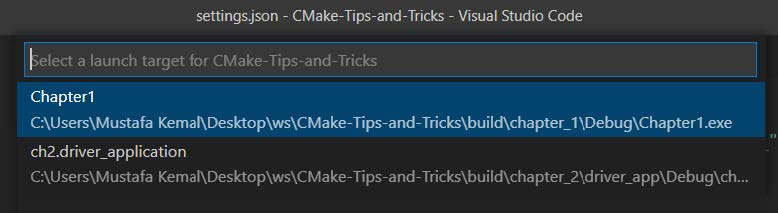
\includegraphics[width=0.8\textwidth]{content/1/chapter2/images/45.jpg}\\
Figure 2.45 – Debug target selection
\end{center}

Select the target and select CMake: Debug (Ctrl + F5) from the Command Palette. The selected target will be started under the debugger.

If you want to run the selected target without the debugger, select CMake: Run Without Debugging (Shift + F5) instead.

\begin{center}
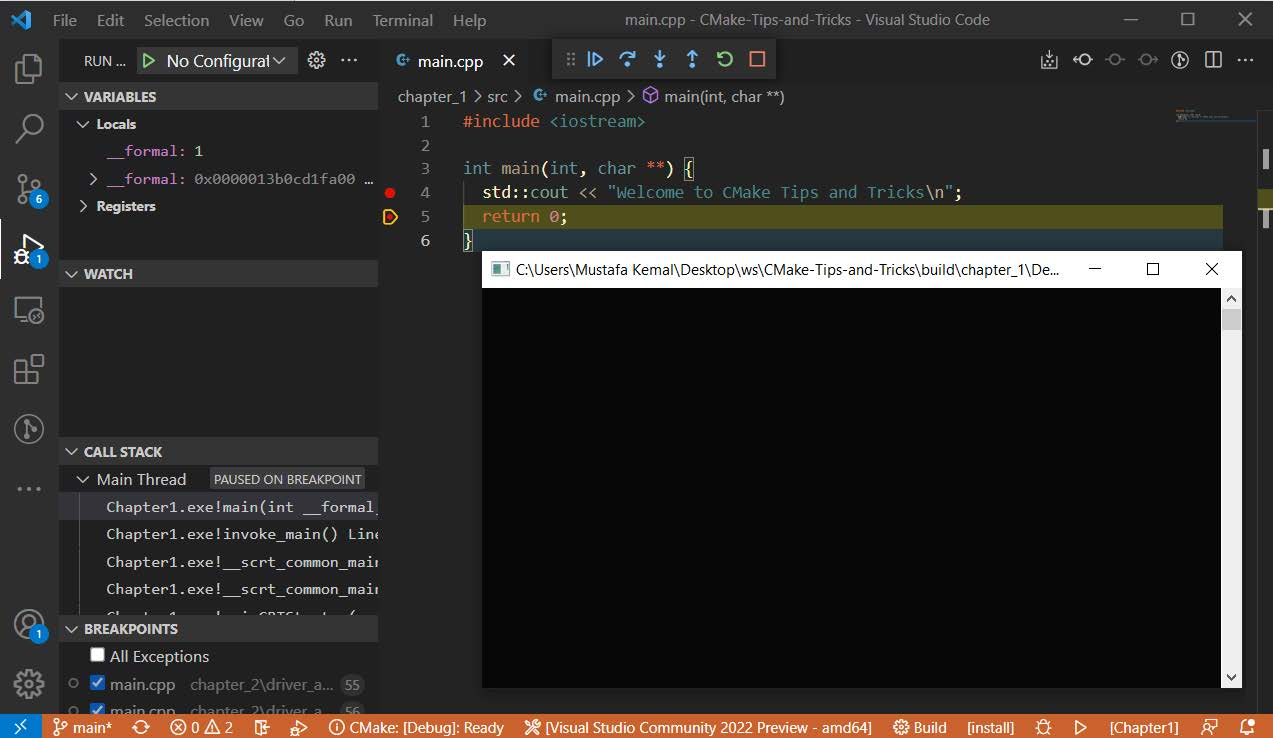
\includegraphics[width=0.8\textwidth]{content/1/chapter2/images/46.jpg}\\
Figure 2.46 – Executable Chapter1 target being debugged
\end{center}

In the next section, we will look at how we can provide arguments to the debugged target.

\hspace*{\fill} \\ %插入空行
\noindent
\textbf{Passing arguments to the debugged target}

The target you're trying to debug might be needing command-line arguments. To pass command-line arguments to the debug target, open VSCode's settings.json file and append the following lines:

\begin{lstlisting}[style=styleCMake]
"cmake.debugConfig": {
		"args": [
		"<argument1>",
		"<argument2>"
		]
	}
\end{lstlisting}

In the args JSON array, you can place any number of arguments your target requires. These arguments will be passed to all future debug targets unconditionally. If you want to have fine-grained control over the arguments, it is better to define a launch.json file instead.

\hspace*{\fill} \\ %插入空行
\noindent
\textbf{Dealing with kits}

A kit in the CMake Tools extension represents a combination of tools that can be used to build the project; hence, the term kit is pretty much a synonym for the toolchain. Kits make it easier to work in a multi-compiler environment, allowing a user to choose which exact compiler to work with. Kits can be discovered automatically by the extension, read from toolchain files, or defined by the user manually.

To see available kits for a project, select the CMake: Select a Kit menu item from the Command Palette (F1 or Ctrl+Shift+P).

\begin{center}
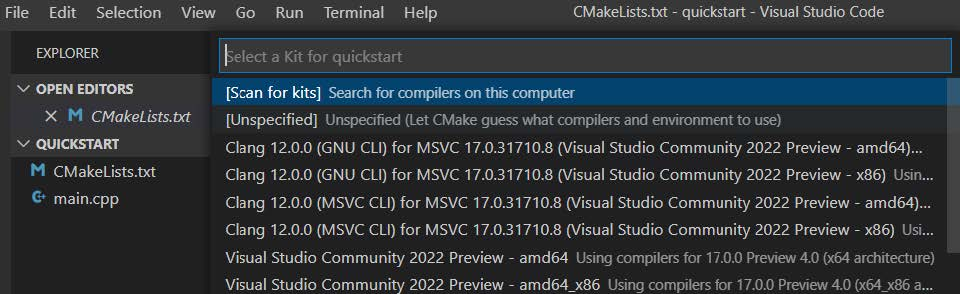
\includegraphics[width=0.8\textwidth]{content/1/chapter2/images/47.jpg}\\
Figure 2.47 – Kit selection list
\end{center}

The selected kit will be used for configuring the CMake project, which means the tools that are defined in the kit will be used for compiling the project. Kit selection will automatically trigger a CMake configuration.

By default, kits are scanned by the extension automatically. As a result, discovered toolchains are listed as options in the kit selection menu. If your toolchain is not displayed here, this means CMake Tools failed to discover it. In such a scenario, try to re-scan for kits first. If it is still missing, you can always define additional kits by adding them to the user-local cmake-tools-kits.json (1) file manually.

Adding a new kit is not usually necessary since the extension does a good job of discovering the toolchains. In the odd case of failure, there is a kit template here, which you can customize and append to the user-local cmake-tools-kits.json file to define a new kit. To open the user-local kits file, select the CMake: Edit User-Local CMake Kits menu item from the Command Palette:

\begin{lstlisting}[style=styleCMake]
{
	"name":"<name of the kit>",
	"compilers" {
		"CXX":"<absolute-path-to-c++-compiler>",
		"C": "<absolute-path-to-c-compiler>"
	}
}
\end{lstlisting}

\begin{tcolorbox}[colback=webgreen!5!white,colframe=webgreen!75!black,title=Note]
In older versions of the CMake Tools extension, the cmake-tools-kits.
json file may be named cmake-kits.json instead.
\end{tcolorbox}

Keep in mind that if your kit name collides with an autogenerated name from CMake Tools, CMake Tools will override your entry on a scan, so, always give unique names to your kit definitions.

For further information about kits, refer to \url{https://github.com/microsoft/vscode-cmake-tools/blob/develop/docs/kits.md}.

\subsubsubsection{2.4.3\hspace{0.2cm}Qt Creator}

Qt Creator is another IDE that supports CMake projects. CMake support is decent and the support comes out of the box without the need for any extra plugins. In this section, we are going to take a quick glance into Qt Creator's CMake support.

As always, ensure that you have the IDE installed and configured properly in your
environment first.

Qt Creator version 5.0.1 is used in the examples.

\hspace*{\fill} \\ %插入空行
\noindent
\textbf{Adding your CMake installation}

In order to use CMake with Qt Creator, the path of CMake must be defined in Qt Creator. To view and define CMake paths, navigate to Tools | Options | Kits | CMake.

\begin{center}
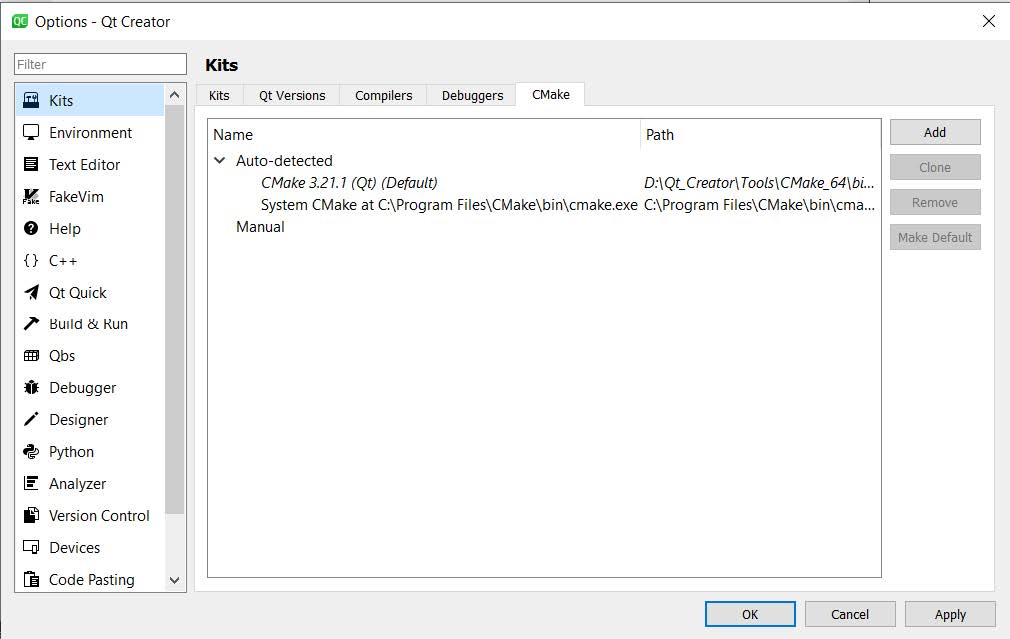
\includegraphics[width=0.8\textwidth]{content/1/chapter2/images/48.jpg}\\
Figure 2.48 – Qt Creator CMake path settings
\end{center}

Albeit with a lack of any manual definition, Qt Creator was able to discover CMake installations in the system. The first entry under the Auto-detected section is the CMake executable shipped together with Qt Creator. The second one is the system's CMake installation. To select which CMake executable to run in Qt Creator, select the desired entry and click the Make Default button.

To add a new CMake executable, click Add. This will append a new entry in the Manual section and bring up a window to fill in the details for the new entry.

\begin{center}
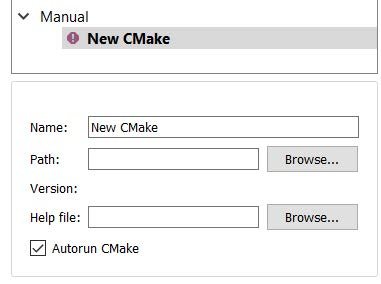
\includegraphics[width=0.6\textwidth]{content/1/chapter2/images/49.jpg}\\
Figure 2.49 – Adding a new CMake executable
\end{center}

The window fields are described in detail here:

\begin{itemize}
\item 
Name: A unique name to distinguish a new CMake executable entry.

\item 
Path: A CMake executable path (cmake/cmake.exe).

\item 
Version: The version of the CMake (deduced by Qt Creator).

\item 
Help file: An optional Qt Creator help file for the executable. This will allow CMake Help to appear upon pressing F1.

\item 
Autorun CMake: Check this to run CMake automatically on any CMakeLists.txt file changes.
\end{itemize}

After filling in the details, click Apply to add the new CMake executable to Qt Creator. Don't forget to set it as default if you intend Qt Creator to use it.

\hspace*{\fill} \\ %插入空行
\noindent
\textbf{Creating a CMake project}

Creating a CMake project in Qt Creator follows the exact same steps as for regular project creation. Qt Creator does not treat CMake as an external build system generator. Instead, it lets its users choose between three build system generators, which are qmake, cmake, and qbs. Any type of Qt project can be started by any of these build system generators from scratch.

To create a CMake project in Qt Creator, click File | New File or Project... (Ctrl + N) and choose the type of project from the New File or Project window. We'll go with Qt Widgets Application for our example.

\begin{center}
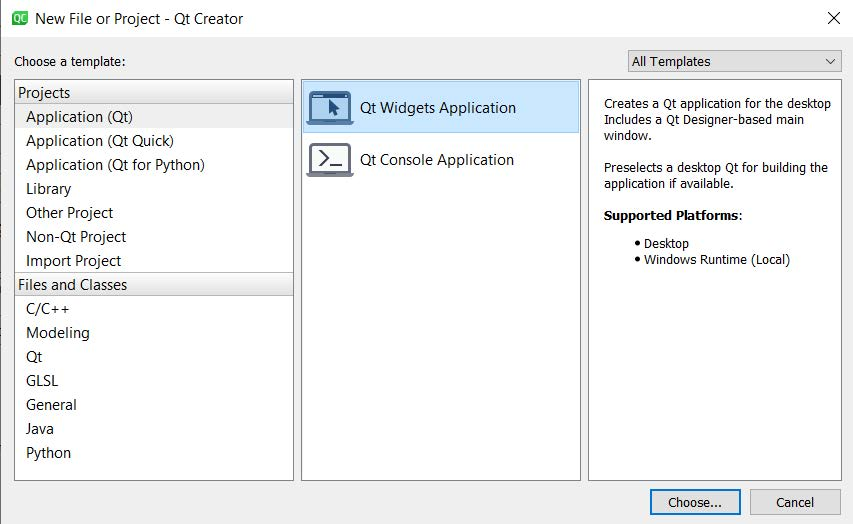
\includegraphics[width=0.8\textwidth]{content/1/chapter2/images/50.jpg}\\
Figure 2.50 – Qt Creator New File or Project window
\end{center}

Upon selection, the project creation wizard will appear. Fill in the details as desired. Select CMake in the Define Build System step, as shown in the following screenshot:

\begin{center}
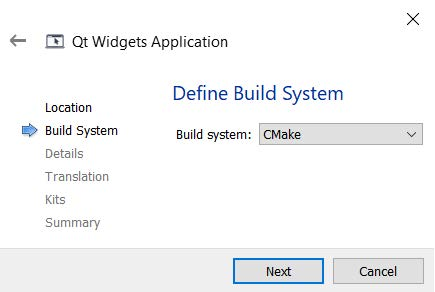
\includegraphics[width=0.6\textwidth]{content/1/chapter2/images/51.jpg}\\
Figure 2.51 – Qt Creator new project wizard build system selection
\end{center}

That's it! You've got yourself a Qt application with the CMake build system.

The following figure shows a newly created CMake project:

\begin{center}
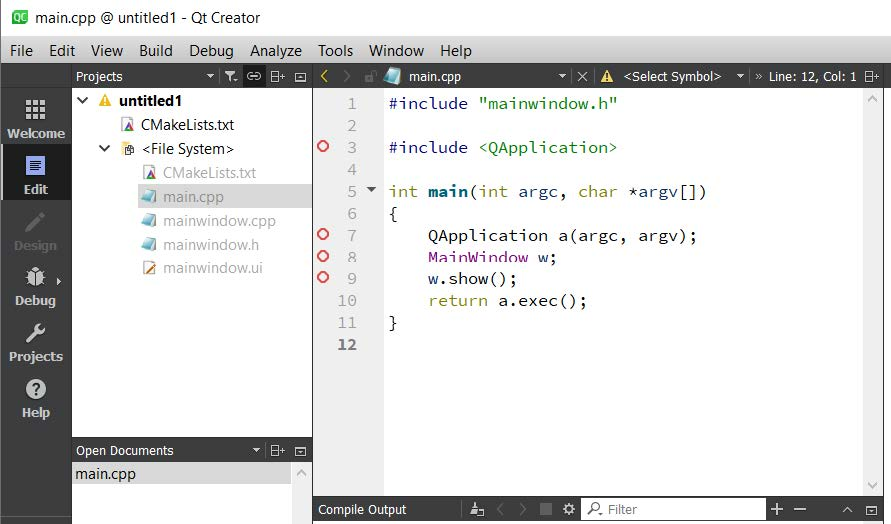
\includegraphics[width=0.8\textwidth]{content/1/chapter2/images/52.jpg}\\
Figure 2.52 – Generated CMake-based Qt widgets application project
\end{center}

\hspace*{\fill} \\ %插入空行
\noindent
\textbf{Opening an existing CMake project}

To open an existing CMake project with Qt Creator, go to the File | Open File or Project... (Ctrl + O) menu item. Select the top-level CMakeLists.txt file of the project and then click Open. Qt Creator will prompt you to choose a kit for your project. Select your preferred kits and then click on the Configure Project button. The project will be open and the CMake configure step will be run with the selected kits.

As an example, the CMake Best Practices project opened with Qt Creator is shown in this figure:

\begin{center}
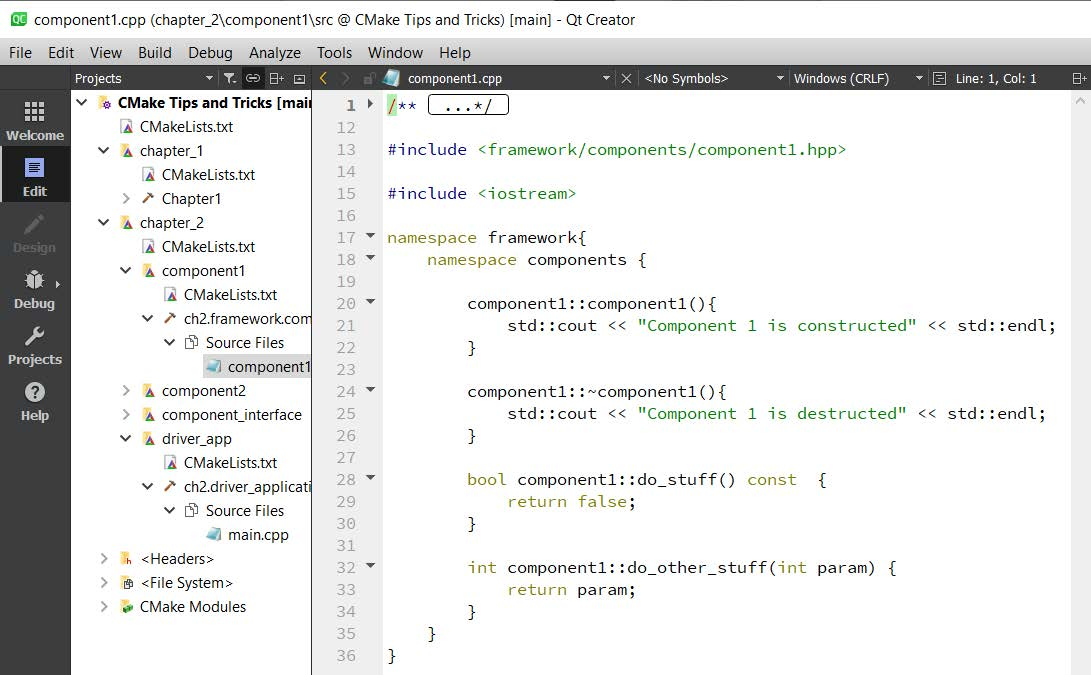
\includegraphics[width=0.8\textwidth]{content/1/chapter2/images/53.jpg}\\
Figure 2.53 – A glance at the CMake Tips and Tricks example project in Qt Creator
\end{center}

After opening a CMake project for the first time, Qt Creator will create a file named CMakeLists.txt.user in the project's root directory. This file contains Qt-specific details that cannot be stored in the CMakeLists.txt file, such as kit information and editor settings.

\hspace*{\fill} \\ %插入空行
\noindent
\textbf{Configuring and building}

In most scenarios (for example, project opening and saving changes to CMakeLists.txt), Qt Creator will run CMake configuration automatically without having to run it manually. To run CMake configuration manually, click on the Build | Run CMake menu item.

After configuration, press the hammer icon in the left-most corner to build the project. Alternatively, the Ctrl + B keyboard shortcut can be used. This will build the whole CMake project. To build a specific CMake target only, use the Locator next to the Build button. Type cm and then press the space bar on your keyboard.

\begin{center}
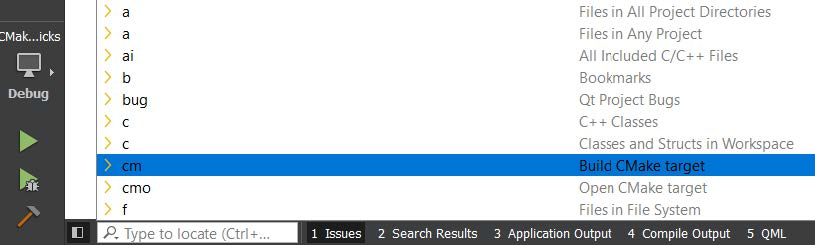
\includegraphics[width=0.8\textwidth]{content/1/chapter2/images/54.jpg}\\
Figure 2.54 – Qt Creator locator suggestions
\end{center}

The locator will display CMake targets available to build. Select the desired target either by highlighting it and pressing Enter, or by clicking on it directly using the mouse.

\begin{center}
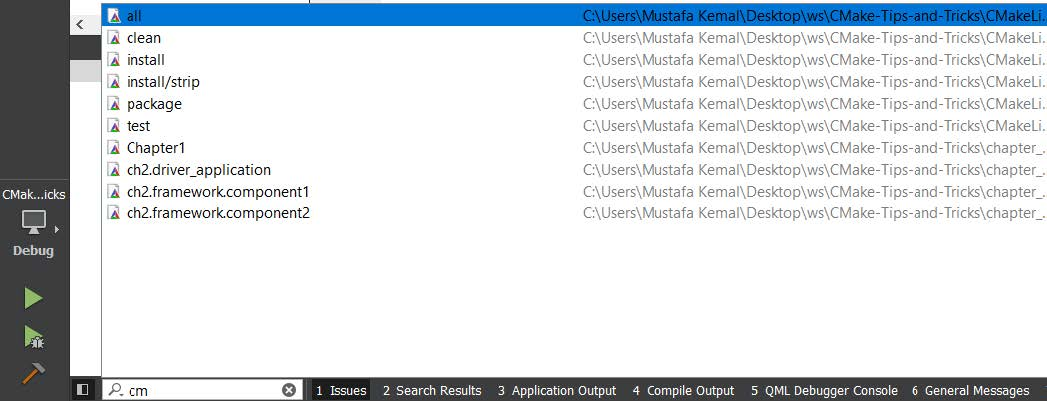
\includegraphics[width=0.8\textwidth]{content/1/chapter2/images/55.jpg}\\
Figure 2.55 – Available CMake targets to build displayed on the locator
\end{center}

The selected CMake target (and naturally, its dependencies) will be built.

\hspace*{\fill} \\ %插入空行
\noindent
\textbf{Run and debug}

To run or debug a CMake target, press the kit selector button (the computer icon on the left navigation bar) and select the CMake target. Then, click either the run button (the play icon under the kit selector) to run or the debug button (the play icon with a bug) to debug.

The following figure shows the kit selector menu content:

\begin{center}
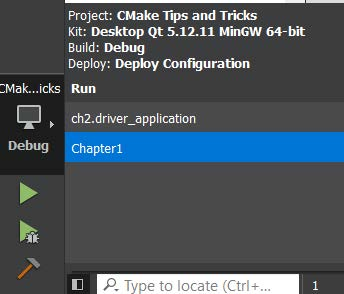
\includegraphics[width=0.5\textwidth]{content/1/chapter2/images/56.jpg}\\
Figure 2.56 – Kit selector displaying CMake targets
\end{center}

Here, we conclude the basics of using CMake with Qt Creator. For more advanced topics, you can consult the resources given in the Further reading section.

















